\documentclass[11pt,a4paper]{article}
\usepackage{iftex}
\ifPDFTeX\usepackage[utf8]{inputenc}\fi
\usepackage[T1]{fontenc}
\usepackage{lmodern}
\usepackage[italian]{babel}
\usepackage[margin=2.2cm,headheight=15pt]{geometry}
\usepackage{amsmath,amssymb,graphicx,booktabs,tabularx,array}
\usepackage{siunitx,xcolor,enumitem,listings,caption,placeins,fancyhdr}
\usepackage[protrusion=true,expansion=false]{microtype}
\usepackage{xurl,hyperref,bookmark}
\definecolor{blu}{RGB}{25,65,105}
\definecolor{grigiochiaro}{RGB}{247,248,250}
\hypersetup{colorlinks=true,linkcolor=blu,citecolor=blu,urlcolor=blu,
  pdftitle={Ricostruzione e georeferenziazione di traiettorie},
  pdfauthor={Lorenzo Maria Alberto Paoria}}
\sisetup{output-decimal-marker={,},group-separator={\,},group-minimum-digits=4,group-digits=integer}
\graphicspath{{figures/}}
\setlength{\parindent}{0pt}
\setlength{\parskip}{4pt}
\setlength{\emergencystretch}{2em}
\setlist{nosep,topsep=4pt}
\renewcommand{\arraystretch}{1.12}
\captionsetup{font=small,labelfont=bf}
\pagestyle{fancy}
\fancyhf{}
\fancyhead[L]{\small Analisi Numerica}
\fancyhead[R]{\small Traiettorie e calibrazione stradale}
\fancyfoot[C]{\thepage}
\lstset{language=Python,basicstyle=\footnotesize\ttfamily,
  keywordstyle=\color{blu},commentstyle=\color{black!55},
  backgroundcolor=\color{grigiochiaro},frame=single,rulecolor=\color{black!15},
  breaklines=true,columns=fullflexible,keepspaces=true,showstringspaces=false,
  aboveskip=5pt,belowskip=6pt}
\newcommand{\norm}[1]{\left\lVert#1\right\rVert}
\newcommand{\slides}[1]{\textit{Dispense di Interpolazione, pp.~#1~\cite{dispense}.}}
\newcommand{\python}{\textbf{Python -- estratto essenziale.}}
\numberwithin{equation}{section}

\title{\color{blu}\bfseries Ricostruzione e georeferenziazione\\di traiettorie da video}
\author{Lorenzo Maria Alberto Paoria\\[3pt]\normalsize Matricola: 1000016111}
\date{\small Progetto di Analisi Numerica\\Prof. Sebastiano Boscarino}

\begin{document}
\maketitle
\thispagestyle{empty}

\section{Obiettivo e dati}

Il progetto confronta i metodi di interpolazione del corso nella
ricostruzione delle posizioni mancanti di automobili riprese da telecamere
fisse. YOLO11n rileva gli oggetti; ByteTrack associa le rilevazioni nel
tempo. Il punto della traiettoria è il \emph{bottom center} della box:
\begin{equation}
 u=\frac{u_{\min}+u_{\max}}{2},\qquad v=v_{\max},\qquad
 P(t)=\begin{bmatrix}u(t)\\v(t)\end{bmatrix}.
\end{equation}
Le box sono dati del rilevatore utilizzati per localizzare l'oggetto;
la grandezza da ricostruire è la traiettoria.

\begin{table}[htbp]
\centering
\caption{Video Urban Tracker elaborati per intero~\cite{urbantracker}.}
\begin{tabular}{lrrr}
\toprule
Video & Frame & Durata circa & Osservazioni YOLO/ByteTrack\\
\midrule
Sherbrooke & \num{4000} & 2 min 13 s & \num{40331}\\
René-Lévesque & \num{8501} & 4 min 44 s & \num{219327}\\
\bottomrule
\end{tabular}
\end{table}

\textbf{Stato del lavoro.}
\begin{itemize}
  \item Confronto in pixel, esperimenti sintetici, clip e video completi:
  eseguiti.
  \item Georeferenziazione: calibrazioni manuali pubblicate e primo
  confronto in metri eseguito su 406 gap nella zona valida; mancano
  checkpoint geografici indipendenti.
  \item Cinematica: valutazione eseguita su 406 gap metrici; il riferimento
  cinematico è una stima da differenze finite della traiettoria completa
  YOLO/ByteTrack e non una ground truth indipendente.
\end{itemize}

Le osservazioni complete sono salvate; alcune vengono poi nascoste agli
interpolatori e usate soltanto dal valutatore. Il riferimento è quindi
YOLO/ByteTrack, non una posizione fisica esatta. Il protocollo è
\emph{post-tracking}: gli identificatori sono già assegnati prima della
rimozione dei campioni.

\section{Concetti del corso utilizzati}

Questo capitolo riassume gli strumenti di Analisi Numerica impiegati nel
progetto. Il capitolo successivo ne presenta formule, condizioni al
contorno ed estratti di implementazione.

\subsection{Strumenti spiegati nelle dispense}

Questa sezione raccoglie i concetti direttamente riconducibili alle
dispense del corso: interpolazione polinomiale, spline, nodi di Chebyshev,
periodicità e interpolazione trigonometrica. Le pagine precise sono
richiamate nel capitolo successivo.

\subsubsection{Interpolazione di dati discreti}

Il problema centrale è ricostruire i valori di una traiettoria nei tempi
in cui l'osservazione è stata rimossa. Dati nodi distinti
$(x_i,y_i)_{i=0}^n$, si cerca una funzione $\widetilde f$ tale che
\[
 \widetilde f(x_i)=y_i,\qquad i=0,\ldots,n.
\]
Nel progetto $x_i$ è il tempo e $y_i$ è una coordinata dell'automobile,
prima in pixel $(u,v)$ e poi, quando la calibrazione è valida, in metri
$(E,N)$. Il riferimento completo viene conservato prima della
mascheratura: i valori nascosti servono solo a misurare l'errore.

\subsubsection{Rappresentazioni polinomiali}

Sono state utilizzate le tre rappresentazioni polinomiali affrontate nel
corso: base monomiale e matrice di Vandermonde, forma di Lagrange e forma
di Newton con differenze divise e schema di Horner. Con gli stessi nodi e
dati esse rappresentano lo stesso polinomio di grado al più $n$; il
confronto separa quindi l'errore di interpolazione dalla formulazione
numerica.

\subsubsection{Spline e condizioni al contorno}

Per limitare le oscillazioni dei polinomi globali sono state considerate
S1 lineare a tratti, S2 quadratica a tratti, S3 naturale, S3 vincolata e
S3 periodica. Le spline cubiche sono $C^2$; la S3 naturale annulla le
derivate seconde agli estremi, mentre la vincolata assegna le derivate
prime. La periodicità richiede valori e derivate compatibili alla chiusura
del periodo. Le condizioni al bordo modificano anche le derivate usate
per la cinematica.

\subsubsection{Nodi, periodicità e interpolazione trigonometrica}

L'esperimento di Runge mostra che i nodi equispaziati possono produrre
oscillazioni elevate, mentre i nodi di Chebyshev riducono l'errore
massimo. Chebyshev è una scelta dei nodi, non una nuova formulazione sugli
stessi dati. Per il segnale sintetico periodico è stata usata anche
l'interpolazione trigonometrica, cioè una combinazione finita di seni e
coseni; con campioni mancanti i coefficienti sono ricavati risolvendo il
sistema sui soli tempi osservati. La periodicità non è imposta ai video
stradali.

\subsection{Estensioni introdotte nel progetto}

La spline quadratica S2 e la costruzione baricentrica di Floater--Hormann
non sono presentate come metodi autonomi principali nelle dispense. S2 è
stata costruita a partire dalla definizione generale di spline
$s^m\in C^{m-1}$, mentre Floater--Hormann è un algoritmo specifico della
famiglia razionale introdotta nel corso. Sono state aggiunte per ampliare
il confronto sperimentale e sono indicate come estensioni anche nelle
tabelle dei risultati.

\subsection{Strumenti applicativi e criteri di valutazione}

\subsubsection{Normalizzazione, stabilità e condizionamento}

I tempi sono trasformati nell'intervallo $[-1,1]$, migliorando la
stabilità del sistema di Vandermonde e rendendo confrontabili i supporti.
Per la base monomiale si registra il numero di condizionamento
$\kappa_2(V_n)$, che misura la sensibilità rispetto a perturbazioni e
arrotondamenti. La scelta della formulazione non elimina invece l'errore
dovuto a un supporto troppo ampio o a troppi nodi.

\subsubsection{Derivazione e grandezze cinematiche}

Velocità e heading non sono interpolati separatamente: si derivano i
modelli delle coordinate,
\[
 v_E(t)=E'(t),\quad v_N(t)=N'(t),\quad
 V(t)=\sqrt{v_E(t)^2+v_N(t)^2},
\]
\[
 \theta(t)=\left[\frac{180}{\pi}\operatorname{atan2}
 (v_E(t),v_N(t))+360\right]\bmod 360.
\]
Le accelerazioni sono le seconde derivate. La regola della catena per i
tempi normalizzati e la regolarità della spline sono quindi parte del
metodo numerico.

\subsubsection{Metriche di errore e confronto}

La valutazione usa i campioni nascosti e due metriche di errore
complementari. Posto
$e_i=\norm{P_i-\widehat P_i}_2$, dove $P_i$ è la posizione di riferimento
e $\widehat P_i$ quella ricostruita, si definiscono
\begin{equation}
 \operatorname{ADE}=\frac1M\sum_{i=1}^{M}e_i,\qquad
 \operatorname{RMS}_{P}=\sqrt{\frac1M\sum_{i=1}^{M}e_i^2}.
\end{equation}
\textbf{ADE} (\emph{Average Displacement Error}) è l'errore medio di
posizione: per ogni campione nascosto si calcola la distanza euclidea tra
la posizione ricostruita e quella di riferimento, poi si fa la media.
Mantiene le stesse unità della posizione, cioè pixel oppure metri, e può
essere interpretato come errore tipico della ricostruzione.

\textbf{RMS} (\emph{Root Mean Square}) è la radice della media dei
quadrati degli errori di posizione. Ha anch'essa unità pixel oppure metri,
ma penalizza maggiormente gli errori grandi perché questi vengono elevati
al quadrato prima della media. È quindi utile per mettere in evidenza
oscillazioni o pochi errori particolarmente elevati. Vale sempre
$\operatorname{RMS}_{P}\geq\operatorname{ADE}$, con uguaglianza quando
tutti gli errori hanno la stessa ampiezza.

Nel progetto ADE e RMS sono calcolati sugli stessi campioni nascosti e
rispetto allo stesso riferimento YOLO/ByteTrack. Non sono quindi misure
assolute dell'errore fisico dell'automobile o della precisione GPS.
Sono inoltre registrati tempi di fit, fallimenti numerici, condizionamento
e copertura. L'errore di ricostruzione è tenuto distinto dall'errore della
calibrazione geografica.

Omografia, DLT, SVD e conversione WGS84 appartengono invece alla
calibrazione del piano stradale, descritta nel capitolo successivo, e non
sono metodi di interpolazione del corso. Analogamente, Python, NumPy,
SciPy e i video sono strumenti di implementazione e di verifica del
progetto, non contenuti teorici aggiuntivi delle dispense.

\section{Calibrazione del piano stradale}

\subsection{Orientamento sulla mappa}
I link geografici pubblicati dal dataset permettono di centrare la mappa
sulle scene. Le coordinate seguenti sono \textbf{centri approssimativi
delle inquadrature}, non posizioni misurate delle telecamere né punti di
controllo da usare automaticamente nel fit.

\begin{center}
\begin{tabular}{lrr}
\toprule
Scena & Latitudine & Longitudine\\
\midrule
Sherbrooke / Atateken, ex Amherst & \num{45.521379} & \num{-73.565683}\\
René-Lévesque Ouest, zona 1425 & \num{45.494921} & \num{-73.574007}\\
\bottomrule
\end{tabular}
\end{center}

\subsection{Omografia}
Un'omografia associa punti dell'immagine a punti di un unico piano.
La calibrazione usa pixel normalizzati e restituisce coordinate locali
nell'ordine Nord--Est:
\begin{equation}
 \begin{bmatrix}\widetilde N\\\widetilde E\\q\end{bmatrix}
 =\mathbf H\begin{bmatrix}u/W\\v/H_{\mathrm{img}}\\1\end{bmatrix},
 \qquad N=\frac{\widetilde N}{q},\quad E=\frac{\widetilde E}{q},\quad q\ne0.
\end{equation}
$W,H_{\mathrm{img}}$ sono le dimensioni del frame. Il progetto usa campi
nominati e fornisce agli interpolatori la coppia $(E,N)$ in metri.
Latitudine e longitudine WGS84 sono ottenute con la conversione locale
della stessa libreria.

\textbf{Procedura operativa.}
\begin{enumerate}
  \item Selezionare alcuni punti riconoscibili sul piano stradale
  nell'immagine e identificarne le coordinate geografiche o metriche
  corrispondenti.
  \item Usare almeno quattro coppie non degeneri, preferibilmente 6--10
  punti ben distribuiti nell'area visibile.
  \item Stimare la matrice omografica con DLT normalizzato e SVD,
  controllando i residui e individuando eventuali outlier.
  \item Verificare la calibrazione su punti di controllo non utilizzati
  nella stima, quindi salvare la matrice e i parametri della scena.
\end{enumerate}

Sono stati pubblicati 7 punti per Sherbrooke, di cui 6 inlier, con RMS
del fit di circa \num{0.280} m, e 4 punti per René-Lévesque, con residuo
numericamente nullo. Non sono ancora stati forniti checkpoint indipendenti.

\python\ L'adattatore richiama l'API condivisa \texttt{GroundProjector}:
\begin{lstlisting}
from src.georeference import GroundCalibration, settings

g = GroundCalibration(settings(), "urban_sherbrooke", 800, 600)
p = g.project((u, v))
E, N = p["east_m"], p["north_m"]
lat, lon = p["latitude_deg"], p["longitude_deg"]
\end{lstlisting}

Il fit condiviso usa DLT normalizzato, SVD e selezione robusta delle
corrispondenze. La proiezione controlla sorgente, preprocessing,
dimensioni e poligono valido. Si considerano soltanto punti del piano
stradale calibrato: tetti, facciate e superfici a quote diverse non sono
descritti dalla stessa omografia.

Il flusso metrico è:
\[
 \text{pixel}\ \longrightarrow\ (E,N)\text{ in metri}\
 \longrightarrow\ \text{interpolazione}\
 \longrightarrow\ (\text{latitudine},\text{longitudine}).
\]
Il residuo sui punti del fit e l'errore su punti indipendenti devono
essere distinti. Quattro corrispondenze possono dare residuo quasi nullo
senza certificare l'accuratezza dell'intera zona.

\section{Metodi: definizione, formula e implementazione}

Si mantiene la notazione delle dispense: $x_i$ sono i \textbf{nodi} e
$y_i$ i valori della coordinata da interpolare. Nel progetto $x_i$
corrisponde al tempo e $y_i$ a $u_i,v_i$ oppure $E_i,N_i$.
Le \textbf{condizioni di interpolazione} sono
\begin{equation}
 \widetilde f(x_i)=y_i,\qquad i=0,\ldots,n.
\end{equation}
Gli estratti mostrano fit e valutazione dal modulo
\path{src/interpolation.py}. Controlli degli input,
gestione degli errori e derivate sono omessi dagli estratti.

\subsection{Preparazione comune dei tempi}
Il tempo viene normalizzato in $[-1,1]$:
\begin{equation}
 \tau=2\frac{t-t_{\min}}{t_{\max}-t_{\min}}-1.
\end{equation}
Nei frammenti, \texttt{x} contiene i nodi normalizzati e \texttt{xq} i
tempi normalizzati da ricostruire. \texttt{y} contiene soltanto valori
visibili. La trigonometrica usa invece direttamente \texttt{t} e
\texttt{tq}, con periodo fisico noto.
\begin{lstlisting}
import numpy as np
from numpy.polynomial import Polynomial
from scipy.interpolate import CubicSpline, PPoly, make_interp_spline

span = t[-1] - t[0]
x = 2 * (t - t[0]) / span - 1
xq = 2 * (tq - t[0]) / span - 1
\end{lstlisting}

\subsection{Interpolazione polinomiale nella base dei monomi}
\slides{7--9}

Si determina un polinomio risolvendo il sistema con \textbf{matrice di
Vandermonde}:
\begin{equation}
 p_n(x)=\sum_{j=0}^{n}a_jx^j,\qquad
 V_n a=y,\qquad (V_n)_{ij}=x_i^j.
\end{equation}
Con $n+1$ nodi distinti esiste un unico polinomio di grado al più $n$.

\python\ \texttt{numpy.vander}, \texttt{numpy.linalg.solve},
\texttt{Polynomial}:
\begin{lstlisting}
V = np.vander(x, N=len(x), increasing=True)
a = np.linalg.solve(V, y)
p = Polynomial(a)
yq = p(xq)
\end{lstlisting}

\subsection{Polinomi di Lagrange}
\slides{10--12}

Il polinomio è una combinazione lineare dei valori $y_i$ e dei polinomi
elementari $L_i$:
\begin{equation}
 p_n(x)=\sum_{i=0}^{n}y_iL_i(x),\qquad
 L_i(x)=\prod_{\substack{j=0\\j\ne i}}^{n}\frac{x-x_j}{x_i-x_j}.
\end{equation}

\python\ Formula diretta, implementata mediante \texttt{numpy.prod}:
\begin{lstlisting}
yq = np.zeros_like(xq, dtype=float)
for i in range(len(x)):
    other = np.delete(x, i)
    denominator = np.prod(x[i] - other)
    Li = np.prod(xq[:, None] - other, axis=1) / denominator
    yq += y[i] * Li
\end{lstlisting}

\subsection{Forma di Newton e differenze divise}
\slides{18--27}

Si costruisce il polinomio mediante \textbf{differenze divise} e lo si
valuta con lo \textbf{schema di Horner}:
\begin{align}
 f[x_i]&=y_i,\qquad
 f[x_0,\ldots,x_k]=
 \frac{f[x_1,\ldots,x_k]-f[x_0,\ldots,x_{k-1}]}{x_k-x_0},\\
 P_n(x)&=f[x_0]+\sum_{k=1}^{n}f[x_0,\ldots,x_k]
 \prod_{i=0}^{k-1}(x-x_i).
\end{align}

\python\ Differenze divise e Horner sono implementati direttamente:
\begin{lstlisting}
d = np.asarray(y, dtype=float).copy()
for k in range(1, len(x)):
    d[k:] = (d[k:] - d[k-1:-1]) / (x[k:] - x[:-k])

yq = np.full_like(xq, d[-1], dtype=float)
for i in range(len(x) - 2, -1, -1):
    yq = d[i] + (xq - x[i]) * yq
\end{lstlisting}

Vandermonde, Lagrange e Newton producono lo stesso polinomio sugli stessi
nodi; cambiano costruzione, valutazione e comportamento numerico.

\subsection{Spline di grado 1: S1}
\slides{36 e 38}

È l'interpolazione lineare a tratti, globalmente continua:
\begin{equation}
 s^1(x)=y_i+\frac{y_{i+1}-y_i}{x_{i+1}-x_i}(x-x_i),
 \qquad x\in[x_i,x_{i+1}].
\end{equation}

\python\ \texttt{scipy.interpolate.make\_interp\_spline}, grado 1:
\begin{lstlisting}
model = make_interp_spline(x, y, k=1)
yq = model(xq)
\end{lstlisting}

\subsection{Spline cubica naturale: S3}
\slides{38--41}

È una funzione cubica a tratti, di classe $C^2$, con derivata seconda
nulla agli estremi:
\begin{align}
 s^3_i(x)&=c_{1,i}+c_{2,i}(x-x_i)+c_{3,i}(x-x_i)^2+c_{4,i}(x-x_i)^3,\\
 D^{(2)}s^3(a)&=D^{(2)}s^3(b)=0.
\end{align}

\python\ \texttt{CubicSpline} con condizione \texttt{natural}:
\begin{lstlisting}
model = CubicSpline(x, y, bc_type="natural", extrapolate=False)
yq = model(xq)
\end{lstlisting}

\subsection{Spline cubica vincolata}
\slides{40}

Impone le derivate prime agli estremi:
\begin{equation}
 D^{(1)}s^3(a)=f'(a),\qquad D^{(1)}s^3(b)=f'(b).
\end{equation}
Nel progetto si stimano queste derivate con polinomi quadratici sui
primi e sugli ultimi tre nodi \emph{visibili}.

\python\ \texttt{Polynomial.fit} e condizioni esplicite in
\texttt{CubicSpline}:
\begin{lstlisting}
left = Polynomial.fit(x[:3], y[:3], 2).deriv()(x[0])
right = Polynomial.fit(x[-3:], y[-3:], 2).deriv()(x[-1])
model = CubicSpline(x, y, bc_type=((1, left), (1, right)),
                    extrapolate=False)
yq = model(xq)
\end{lstlisting}

\subsection{Spline cubica periodica}
\slides{40}

È usata per dati periodici con valori compatibili agli estremi:
\begin{equation}
 y_0=y_n,\qquad
 D^{(1)}s^3(a)=D^{(1)}s^3(b),\qquad
 D^{(2)}s^3(a)=D^{(2)}s^3(b).
\end{equation}

\python\ \texttt{CubicSpline} con condizione \texttt{periodic}:
\begin{lstlisting}
# The support spans a complete period and y[0] == y[-1].
model = CubicSpline(x, y, bc_type="periodic", extrapolate=False)
yq = model(xq)
\end{lstlisting}
È verificata nel test sintetico periodico, non forzata sui passaggi
stradali non periodici.

\subsection{Spline quadratica S2: estensione}
La definizione generale delle dispense è $s^m\in C^{m-1}$ (p.~37).
S2 è la costruzione aggiuntiva con $m=2$:
\begin{equation}
 s^2_i(x)=a_i+b_i(x-x_i)+c_i(x-x_i)^2,\qquad s^2\in C^1.
\end{equation}
Posti $h_i=x_{i+1}-x_i$ e $\delta_i=(y_{i+1}-y_i)/h_i$, si usa
\begin{equation}
 a_i=y_i,\quad b_0=\delta_0,\quad
 c_i=\frac{\delta_i-b_i}{h_i},\quad b_{i+1}=b_i+2c_i h_i.
\end{equation}
La condizione aggiuntiva è $c_0=0$.

\python\ Coefficienti costruiti direttamente e valutazione con \texttt{PPoly}:
\begin{lstlisting}
h = np.diff(x)
slopes = np.diff(y) / h
b, c = np.empty_like(h), np.empty_like(h)
b[0] = slopes[0]
for i in range(len(h)):
    c[i] = (slopes[i] - b[i]) / h[i]
    if i + 1 < len(h):
        b[i + 1] = b[i] + 2 * c[i] * h[i]
model = PPoly(np.vstack((c, b, y[:-1])), x, extrapolate=False)
yq = model(xq)
\end{lstlisting}

\subsection{Nodi di Chebyshev}
\slides{28--32}

Sono gli zeri dei polinomi di Chebyshev; per grado interpolante al più
$n$ si usano gli $n+1$ zeri di $T_{n+1}$:
\begin{equation}
 T_k(x)=\cos(k\arccos x),\qquad
 x_j=\cos\left(\frac{(2j+1)\pi}{2(n+1)}\right),\quad j=0,\ldots,n.
\end{equation}
Il cambiamento di intervallo è $t_j=(b-a)x_j/2+(a+b)/2$.

\python\ Generazione con \texttt{numpy.cos}; nel test si valuta la
forma di Newton:
\begin{lstlisting}
from src.interpolation import NewtonPolynomial

j = np.arange(n + 1)
x = np.sort(np.cos((2 * j + 1) * np.pi / (2 * (n + 1))))
y = 1 / (1 + 25 * x**2)
yq = NewtonPolynomial(x, y)(xq)
\end{lstlisting}
Chebyshev è una scelta dei nodi, non una formulazione diversa sugli
stessi dati. Il test dedicato usa la funzione di Runge normalizzata.

\subsection{Interpolazione trigonometrica}
\slides{4 e 6}

È una combinazione di armoniche. Nella forma delle dispense:
\begin{equation}
 \widetilde f(x)=a_{-M}e^{-\mathrm{i}Mx}+\cdots+a_0+\cdots+a_Me^{\mathrm{i}Mx}.
\end{equation}
Per $N=2M+1$ dati, la forma reale con periodo $T$ è
\begin{equation}
 p(t)=a_0+\sum_{k=1}^{M}\bigl[a_k\cos(k\phi(t))+b_k\sin(k\phi(t))\bigr],
 \qquad \phi(t)=\frac{2\pi(t-t_0)}{T}.
\end{equation}
Per $N=2M$ la somma termina a $M-1$ e si aggiunge il solo termine
$a_M\cos(M\phi(t))$. L'estremo finale duplicato è escluso.

\python\ Matrice seno/coseno e \texttt{numpy.linalg.solve}:
\begin{lstlisting}
N = len(t)
def design(times):
    phi = 2 * np.pi * (times - t0) / T
    columns = [np.ones_like(times)]
    for k in range(1, (N - 1) // 2 + 1):
        columns.extend([np.cos(k * phi), np.sin(k * phi)])
    if N % 2 == 0:
        columns.append(np.cos((N // 2) * phi))
    return np.column_stack(columns)

coefficients = np.linalg.solve(design(t), y)
yq = design(tq) @ coefficients
\end{lstlisting}
Con campioni mancanti si risolve il sistema sui tempi osservati;
non si applica direttamente una FFT a una griglia incompleta.

\subsection{Interpolazione razionale: costruzione Floater--Hormann}
La famiglia $r(x)=P(x)/Q(x)$ è introdotta a pagina 4 delle dispense.
L'implementazione specifica è un'estensione~\cite{floater-hormann}:
\begin{equation}
 r(x)=\frac{\displaystyle\sum_{i=0}^{n}\frac{w_i y_i}{x-x_i}}
 {\displaystyle\sum_{i=0}^{n}\frac{w_i}{x-x_i}},\qquad r(x_i)=y_i,
\end{equation}
con $d=\min(3,n)$ e
\begin{equation}
 w_i=(-1)^{i-d}\sum_{j=\max(0,i-d)}^{\min(i,n-d)}
 \prod_{\substack{k=j\\k\ne i}}^{j+d}\frac{1}{|x_i-x_k|}.
\end{equation}

\python\ Pesi e rapporto baricentrico calcolati con NumPy:
\begin{lstlisting}
N, d = len(x), min(3, len(x) - 1)
w = np.zeros(N)
for i in range(N):
    for j in range(max(0, i-d), min(i, N-d-1) + 1):
        indices = [k for k in range(j, j+d+1) if k != i]
        w[i] += 1 / np.prod(np.abs(x[i] - x[indices]))
    w[i] *= (-1.0)**(i-d)
w /= np.max(np.abs(w))

def value(z):
    hit = np.flatnonzero(z == x)
    if len(hit):
        return y[hit[0]]
    terms = w / (z - x)
    return (terms @ y) / terms.sum()

yq = np.array([value(z) for z in xq])
\end{lstlisting}

\section{Protocollo di confronto}

Il riferimento completo è salvato prima di mascherare i dati. I gap
contengono 3, 6, 12, 24, 48, 72, 120 o 240 frame nascosti; ogni fit usa quattro nodi visibili
prima e quattro dopo. I campioni nascosti non diventano supporto di altri
gap. Gli stessi casi sono utilizzati da tutti i metodi.

\begin{lstlisting}
# Essential scheme from src/benchmark.py
from src.interpolation import Interpolator

visible = mask["visible_indices"]
hidden = mask["hidden_indices"]
model_u = Interpolator(method).fit(times[visible], u[visible])
model_v = Interpolator(method).fit(times[visible], v[visible])
predicted = np.column_stack([
    model_u.predict(times[hidden]),
    model_v.predict(times[hidden]),
])
reference = np.column_stack([u[hidden], v[hidden]])
error = np.linalg.norm(predicted - reference, axis=1)
\end{lstlisting}

Per il confronto metrico la coppia $(u,v)$ viene sostituita da $(E,N)$
\emph{prima} del fit. Sono ammissibili soltanto i gap per cui tutti i nodi
di supporto e i riferimenti nascosti hanno una proiezione valida.
La baseline in pixel viene ripetuta su quello stesso sottoinsieme.

\textbf{Metriche.} Si usano ADE e RMS definiti nel Capitolo 2 sugli stessi
campioni nascosti e rispetto allo stesso riferimento.
Si registrano anche tempi, fallimenti e, per la base monomiale,
$\kappa_2(V_n)$. L'errore di ricostruzione in metri rispetto al segnale
proiettato non è una misura indipendente dell'accuratezza GPS dell'auto.

\section{Risultati disponibili}

Il confronto in pixel contiene \num{2148} gap, \num{70485} campioni
nascosti e otto metodi: \num{17184} valutazioni, senza fallimenti numerici.
Le prime tabelle descrivono il run completo in pixel; il confronto
metrico successivo usa il sottoinsieme coperto dalle calibrazioni.

\begin{table}[htbp]
\centering
\caption{ADE in pixel per tutti i gap del benchmark, con otto nodi visibili.}
\scriptsize
\resizebox{\linewidth}{!}{%
\begin{tabular}{l*{8}{S[table-format=4.4]}}
\toprule
Metodo & {3} & {6} & {12} & {24} & {48} & {72} & {120} & {240}\\
\midrule
S1 & 0.3513 & 0.5705 & 0.7855 & 1.2413 & 2.9898 & 4.8868 & 7.8804 & 11.0161\\
Vandermonde & 0.5088 & 1.1545 & 4.2135 & 18.9447 & 101.8808 & 277.0082 & 1142.5919 & 6819.7511\\
Lagrange & 0.5088 & 1.1545 & 4.2135 & 18.9447 & 101.8808 & 277.0082 & 1142.5919 & 6819.7511\\
Newton & 0.5088 & 1.1545 & 4.2135 & 18.9447 & 101.8808 & 277.0082 & 1142.5919 & 6819.7511\\
S3 naturale & 0.3891 & 0.6400 & 1.0348 & 1.8345 & 3.4431 & 5.0748 & 7.5183 & 11.1780\\
S3 vincolata & 0.3890 & 0.6402 & 1.0361 & 1.8365 & 3.4446 & 5.0817 & 7.5269 & 11.1840\\
S2 (estensione) & 0.8633 & 1.4999 & 2.3394 & 4.5059 & 8.4972 & 11.7482 & 19.0089 & 25.8366\\
Razionale FH (estensione) & 0.8018 & 2.2159 & 9.4936 & 46.4790 & 261.9474 & 718.3288 & 3029.1047 & 18220.9100\\
\bottomrule
\end{tabular}
}
\end{table}

\begin{table}[htbp]
\centering
\caption{RMS in pixel per tutti i gap del benchmark, con otto nodi visibili.}
\scriptsize
\resizebox{\linewidth}{!}{%
\begin{tabular}{l*{8}{S[table-format=5.4]}}
\toprule
Metodo & {3} & {6} & {12} & {24} & {48} & {72} & {120} & {240}\\
\midrule
S1 & 0.6301 & 1.3533 & 1.7770 & 3.1589 & 8.8722 & 14.4159 & 21.9145 & 27.1348\\
Vandermonde & 0.6983 & 1.7492 & 10.5720 & 33.4093 & 188.7232 & 488.6295 & 2341.3403 & 11704.6460\\
Lagrange & 0.6983 & 1.7492 & 10.5720 & 33.4093 & 188.7232 & 488.6295 & 2341.3403 & 11704.6460\\
Newton & 0.6983 & 1.7492 & 10.5720 & 33.4093 & 188.7232 & 488.6295 & 2341.3403 & 11704.6460\\
S3 naturale & 0.5445 & 1.0909 & 2.1612 & 2.9122 & 7.0166 & 9.9057 & 15.4943 & 19.0938\\
S3 vincolata & 0.5444 & 1.0908 & 2.1687 & 2.9180 & 7.0139 & 9.9186 & 15.4940 & 19.1123\\
S2 (estensione) & 1.2397 & 2.4729 & 3.7042 & 7.5374 & 14.8758 & 22.0471 & 39.8497 & 45.8191\\
Razionale FH (estensione) & 1.1072 & 3.3968 & 26.2621 & 85.8264 & 516.9439 & 1343.7377 & 6577.1603 & 33259.4248\\
\bottomrule
\end{tabular}
}
\end{table}

Vandermonde, Lagrange e Newton differiscono fra loro al massimo di circa
$10^{-10}$ pixel. I grandi errori sui gap lunghi non si eliminano
cambiando soltanto la formulazione dello stesso polinomio.

Il risultato a favore di S1 è coerente con la natura dei dati: le posizioni
YOLO/ByteTrack sono rumorose e, nei brevi intervalli analizzati, il moto
proiettato è spesso localmente quasi lineare. La S3 stima anche la curvatura
e può quindi introdurre overshoot quando la curvatura è determinata dal
rumore o dalle condizioni al bordo. In questo caso la maggiore regolarità
della cubica non compensa la maggiore sensibilità, mentre S1 privilegia una
ricostruzione locale più robusta.

\begin{table}[htbp]
\centering
\caption{Studio ufficiale dei gap lunghi: confronto diretto fra S1 e S3 naturale.}
\begin{tabular}{l c S[table-format=2.4] S[table-format=2.4]}
\toprule
Gap & Metodo & {ADE (px)} & {RMS (px)}\\
\midrule
48 & S1 & 2.9898 & 8.8722\\
48 & S3 naturale & 3.4431 & 7.0166\\
72 & S1 & 4.8868 & 14.4159\\
72 & S3 naturale & 5.0748 & 9.9057\\
120 & S1 & 7.8804 & 21.9145\\
120 & S3 naturale & 7.5183 & 15.4943\\
240 & S1 & 11.0161 & 27.1348\\
240 & S3 naturale & 11.1780 & 19.0938\\
\bottomrule
\end{tabular}
\end{table}

L'estensione ai gap di 48, 72, 120 e 240 frame mostra che la S3 naturale
può superare S1 sui gap molto lunghi: ottiene ADE minore a 120 frame e RMS
minore in tutti i quattro casi. S1 resta migliore in ADE a 48, 72 e 240
frame. Il risultato non contraddice il benchmark principale: sui dati
rumorosi la S1 è più robusta in media, mentre su intervalli molto estesi la
regolarità della S3 può ridurre gli errori estremi, pur potendo introdurre
overshoot.

\begin{figure}[htbp]
\centering
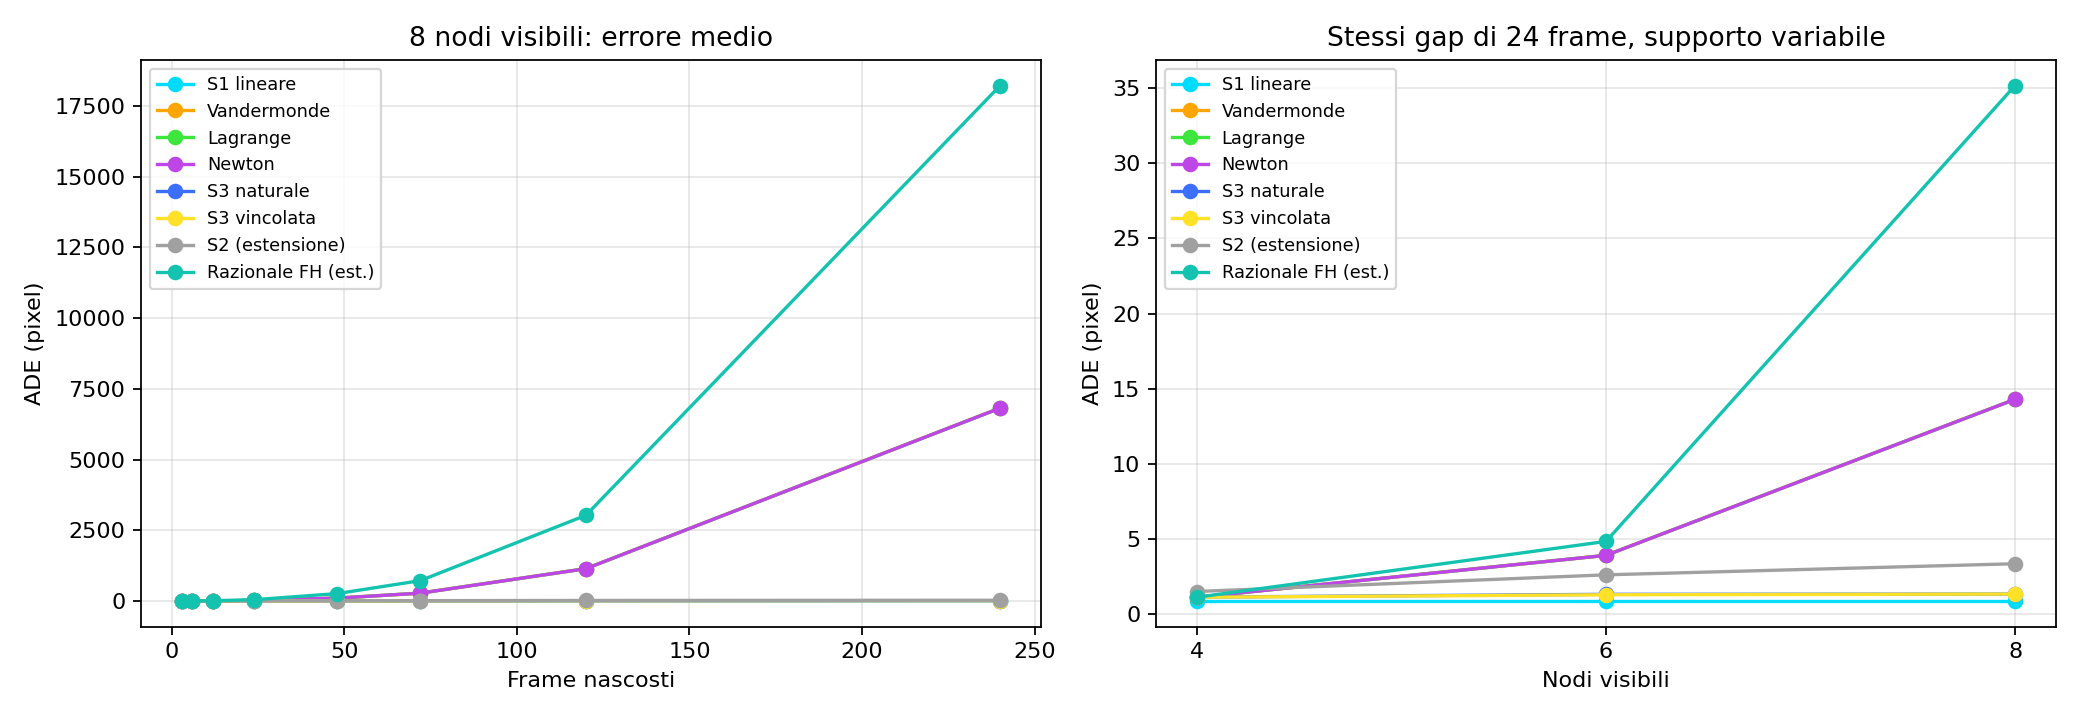
\includegraphics[width=\linewidth]{course_comparison.png}
\caption{Errori al variare di lunghezza del gap e numero di nodi.}
\end{figure}

\subsection{Confronto sul piano stradale calibrato}
Le calibrazioni permettono di proiettare \num{2186} osservazioni di
Sherbrooke e \num{7345} di René-Lévesque. Il dominio valido copre una
parte delle immagini: \textbf{406 gap su \num{5517}} hanno tutti i supporti
e i riferimenti nella zona calibrata; gli altri \num{5111} sono esclusi
dal confronto metrico.

\begin{table}[htbp]
\centering
\caption{Confronto metrico sui 406 gap ammissibili: ADE/RMS per lunghezza del gap.}
\scriptsize
\resizebox{\linewidth}{!}{%
\begin{tabular}{l*{8}{S[table-format=2.4]}}
\toprule
Metodo & \multicolumn{2}{c}{3 frame} & \multicolumn{2}{c}{6 frame} &
\multicolumn{2}{c}{12 frame} & \multicolumn{2}{c}{24 frame}\\
 & {ADE} & {RMS} & {ADE} & {RMS} & {ADE} & {RMS} & {ADE} & {RMS}\\
\midrule
S1 & 0.0450 & 0.0641 & 0.0642 & 0.0967 & 0.0878 & 0.1427 & 0.1075 & 0.1644\\
Vandermonde / Lagrange / Newton & 0.0749 & 0.0970 & 0.1505 & 0.2155 & 0.5576 & 0.8323 & 2.1672 & 3.4613\\
S3 naturale & 0.0570 & 0.0751 & 0.0810 & 0.1102 & 0.1386 & 0.2034 & 0.1987 & 0.2979\\
S3 vincolata & 0.0570 & 0.0751 & 0.0810 & 0.1101 & 0.1386 & 0.2035 & 0.1992 & 0.2989\\
S2 (estensione) & 0.1231 & 0.1674 & 0.1970 & 0.3011 & 0.3548 & 0.5102 & 0.4884 & 0.7782\\
Razionale FH (estensione) & 0.1166 & 0.1523 & 0.2885 & 0.4474 & 1.2840 & 1.9835 & 5.1797 & 9.1738\\
\bottomrule
\end{tabular}
}
\end{table}

La baseline in pixel è ricalcolata su questi stessi casi. Per gap di
24 frame, ad esempio, S1 ha ADE \num{2.0543} pixel nella baseline abbinata
e \num{0.1075} m nel fit metrico. Le grandezze non si convertono mediante
un unico fattore: proiezione e interpolazione non sono operazioni commutative.
Il riferimento in metri resta la proiezione di YOLO/ByteTrack, non un GPS
indipendente dell'automobile.

\begin{figure}[htbp]
\centering
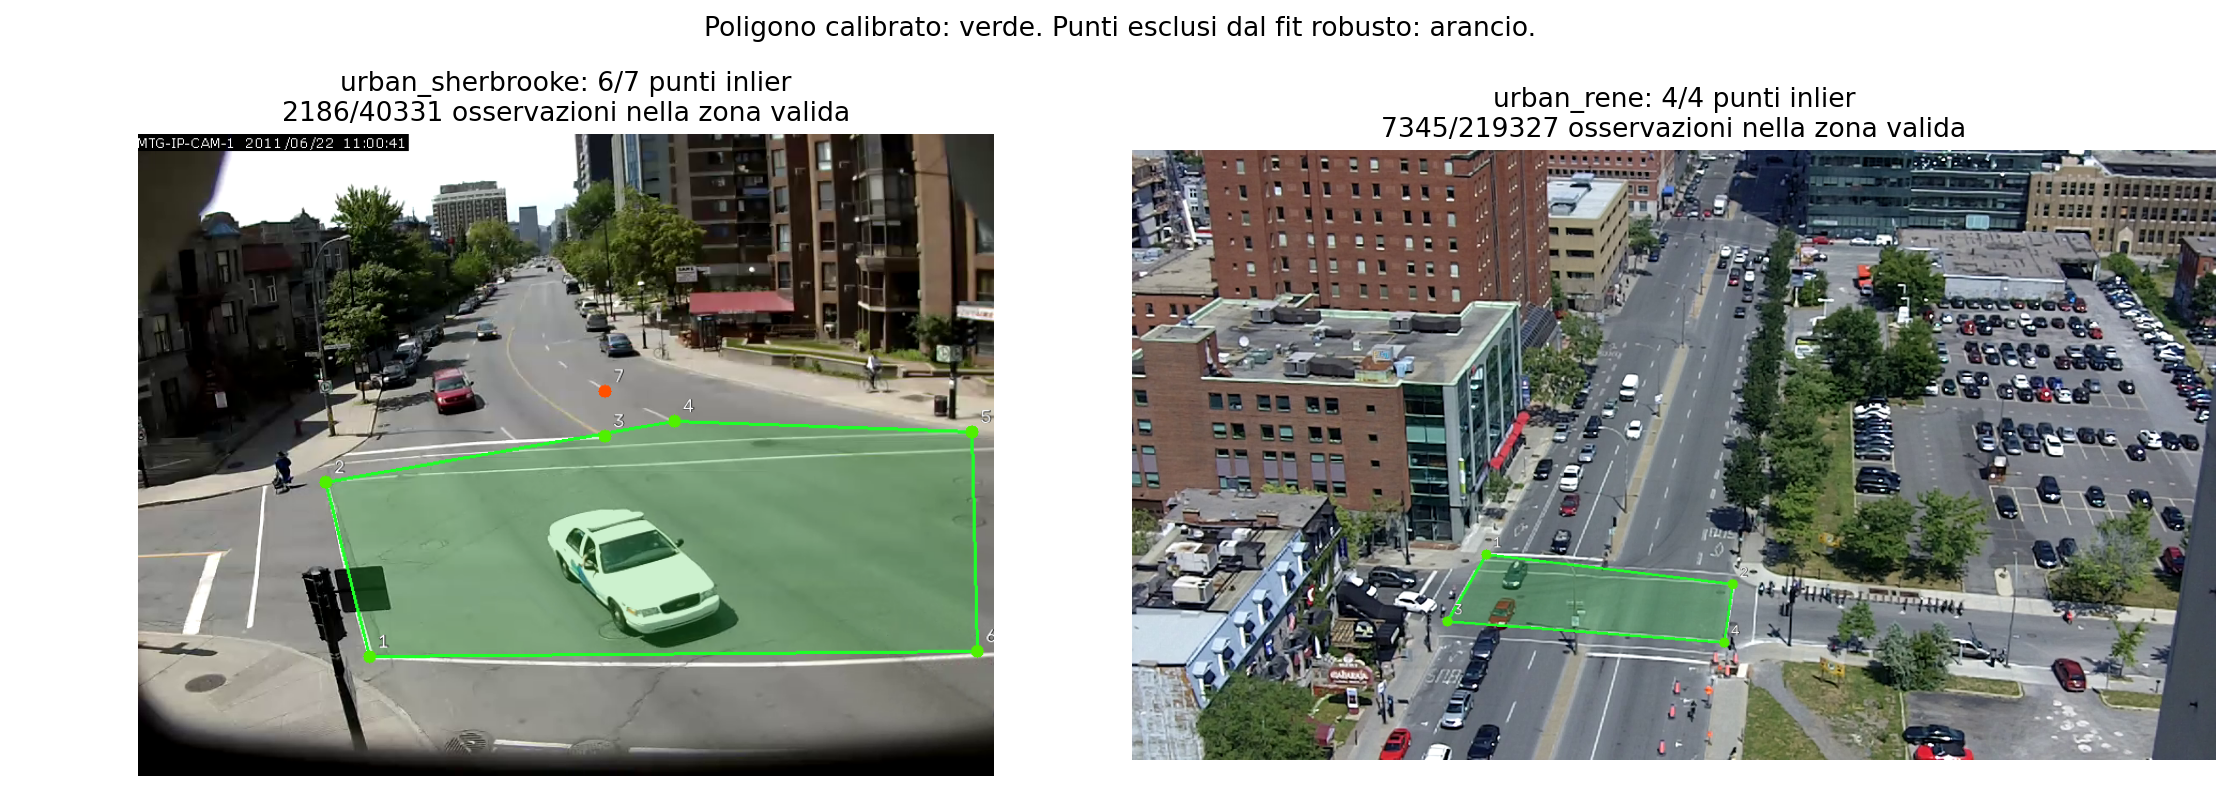
\includegraphics[width=\linewidth]{calibration_coverage.png}
\caption{Zone calibrate in verde e punti usati nel fit. L'arancio indica una corrispondenza esclusa dal fit robusto.}
\end{figure}

\subsection{Esperimenti sintetici}
\textbf{Runge e Chebyshev.} Si interpola
$f(x)=1/(1+25x^2)$ su $[-1,1]$. A grado 32, l'errore massimo è circa
\num{5058.96} sui nodi equispaziati e \num{0.001402} sulle radici di
Chebyshev. La distribuzione dei nodi è determinante.

\textbf{Periodicità.} Si usa, con $T=6$ secondi,
\begin{equation}
 P(t)=\begin{bmatrix}
 12\cos(2\pi t/T)+1.5\cos(4\pi t/T)\\
 8\sin(2\pi t/T)
 \end{bmatrix}.
\end{equation}
Si nascondono otto campioni fra 49, in tre collocazioni. S3 periodica
raggiunge ADE di circa \num{0.0274}--\num{0.0379}; la trigonometrica errori
dell'ordine di $10^{-9}$, perché il segnale appartiene alla base scelta.
Queste unità sintetiche non vengono mescolate ai risultati stradali.

\begin{figure}[htbp]
\centering
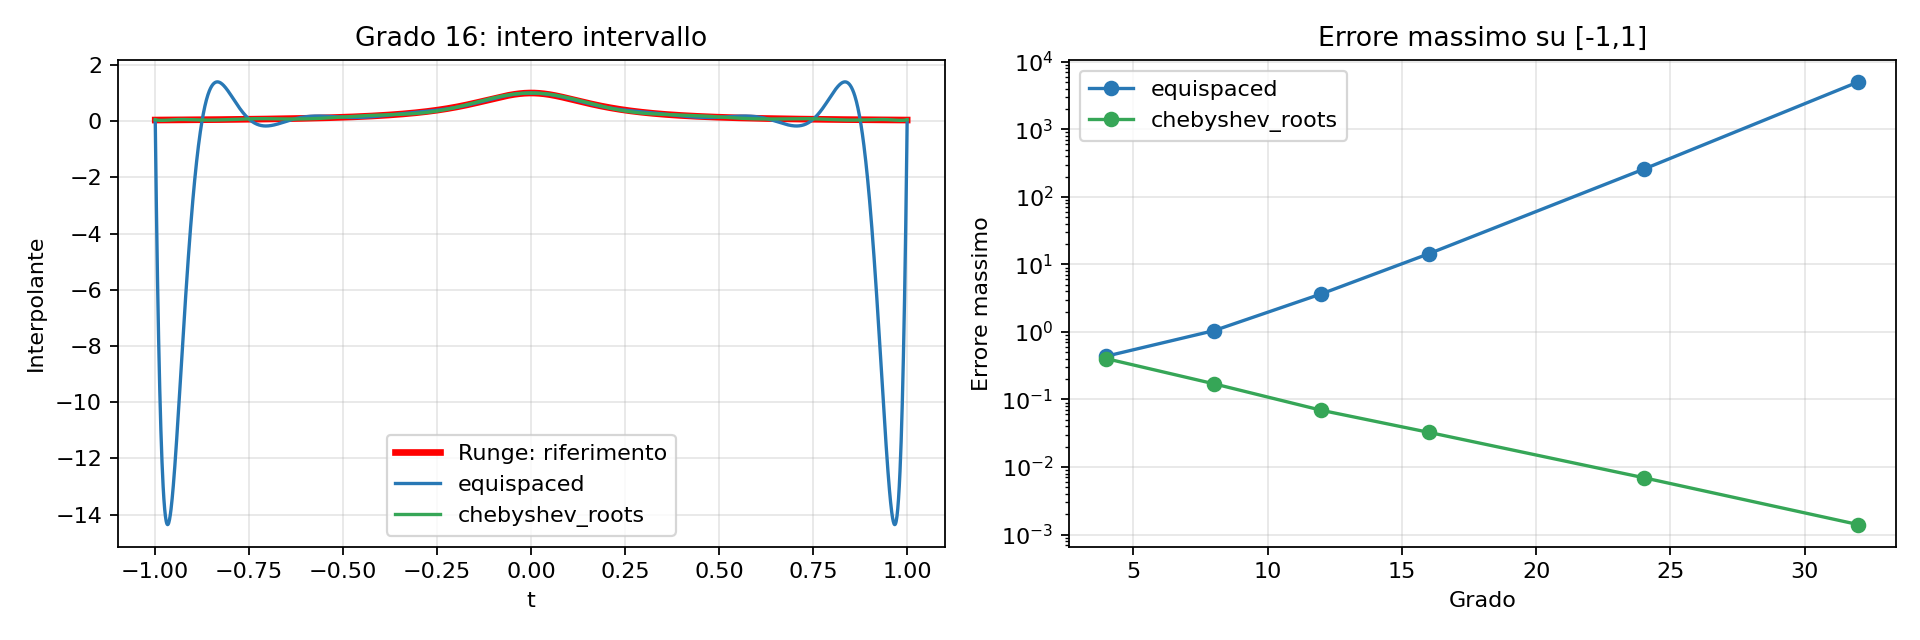
\includegraphics[width=0.95\linewidth]{chebyshev_runge.png}
\caption{Funzione di Runge e scelta dei nodi.}
\end{figure}

\subsection{Clip dei passaggi}
Sono disponibili 12 clip separate, di circa 6,4--8 secondi. Il
riferimento YOLO/ByteTrack è rosso acceso; otto riquadri affiancati
mostrano gli interpolatori con colori distinti. Zoom e istanti nascosti
sono uguali per tutti. La selezione usa movimento e distribuzione
temporale, non gli errori ottenuti. Codifica GPU con NVIDIA NVENC.

I video completi con la ricostruzione sono:
\begin{itemize}
  \item \href{../generated/static_full/full_reconstruction_urban_rene.mp4}
  {Urban René-Lévesque} (8501 frame, circa 4 min 44 s);
  \item \href{../generated/static_full/full_reconstruction_urban_sherbrooke.mp4}
  {Urban Sherbrooke} (4000 frame, circa 2 min 13 s).
\end{itemize}
L'indice delle clip brevi e i relativi file sono nella directory
\texttt{reports/generated/course/clips/}.

\begin{figure}[htbp]
\centering
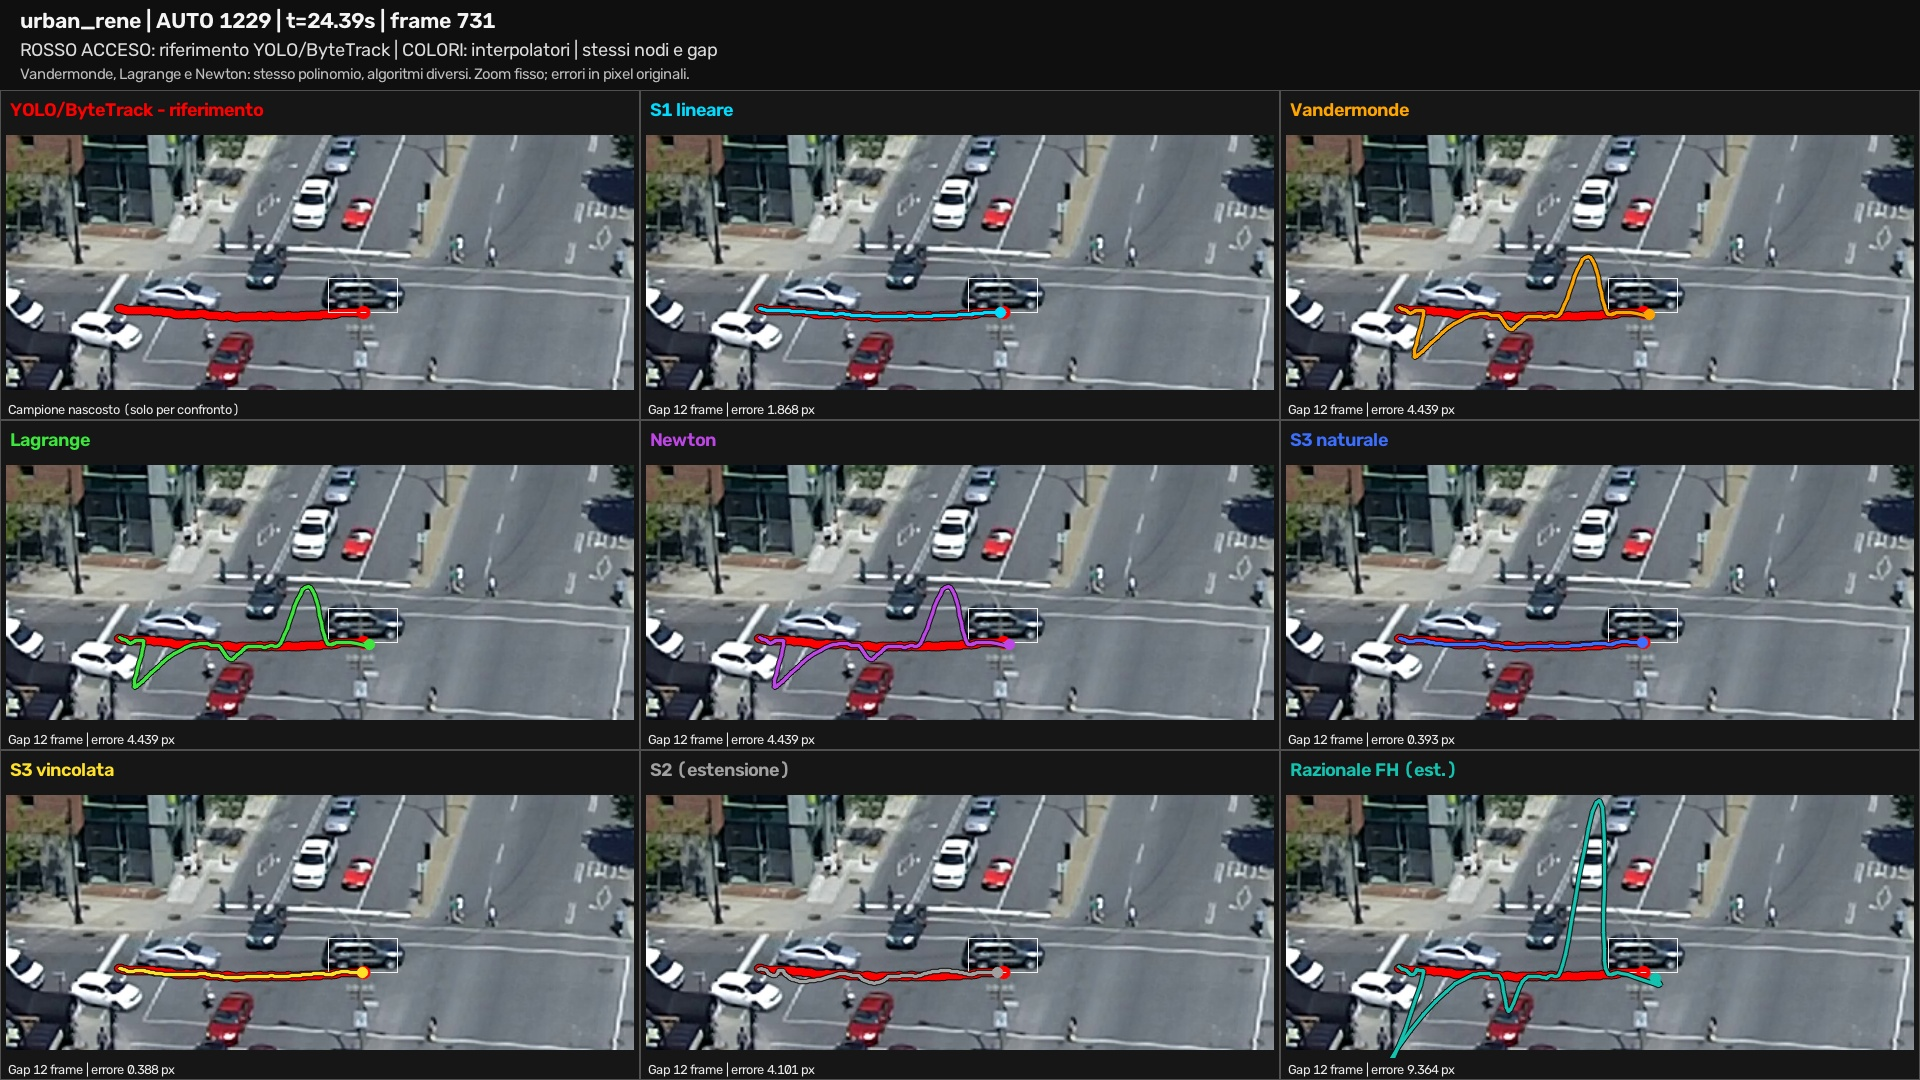
\includegraphics[width=\linewidth]{clip_rene.jpg}
\caption{Stesso passaggio, riferimento rosso e otto interpolatori. Immagini Urban Tracker, elaborazione del progetto.}
\end{figure}

\FloatBarrier
\section{Cinematica}

Velocità, accelerazione e heading si ricavano dagli stessi modelli interpolanti
usati per le coordinate $E(t)$ e $N(t)$:
\begin{equation}
 \mathbf v(t)=\begin{bmatrix}\dot E(t)\\\dot N(t)\end{bmatrix},\qquad
 V(t)=\sqrt{\dot E(t)^2+\dot N(t)^2},\qquad
 \mathbf a(t)=\begin{bmatrix}\ddot E(t)\\\ddot N(t)\end{bmatrix}.
\end{equation}
L'heading, in gradi orari dal Nord, è
\begin{equation}
 \theta(t)=\left[\frac{180}{\pi}\operatorname{atan2}(\dot E(t),\dot N(t))+360\right]\bmod360.
\end{equation}
Quindi non si costruisce un interpolatore separato per la velocità o per
l'heading: si interpola la posizione, si derivano i due modelli e si
calcolano velocità e heading dalle derivate. In particolare, la velocità
è il modulo della derivata e l'heading è l'angolo del vettore velocità;
quest'ultimo va escluso o marcato non definito quando la velocità è
troppo bassa. Il metodo di interpolazione scelto per $E,N$ determina
pertanto anche la regolarità delle grandezze cinematiche.
Il codice dispone già delle derivate e applica la regola della catena:
\begin{equation}
 \frac{d}{dt}=\frac{2}{t_{\max}-t_{\min}}\frac{d}{d\tau},\qquad
 \frac{d^2}{dt^2}=\left(\frac{2}{t_{\max}-t_{\min}}\right)^2\frac{d^2}{d\tau^2}.
\end{equation}

\textbf{Schema Python della fase futura}, non risultato già misurato:
\begin{lstlisting}
model_E = Interpolator(method).fit(t_visible, E_visible)
model_N = Interpolator(method).fit(t_visible, N_visible)
vE = model_E.derivative(tq, order=1)
vN = model_N.derivative(tq, order=1)
aE = model_E.derivative(tq, order=2)
aN = model_N.derivative(tq, order=2)
speed_mps = np.hypot(vE, vN)
heading = (np.degrees(np.arctan2(vE, vN)) + 360) % 360
heading[speed_mps < speed_min] = np.nan
\end{lstlisting}
La valutazione è stata eseguita sui 406 gap metrici già validi. Per ogni
gap si interpolano soltanto i punti visibili, si calcolano le derivate in
tempo fisico e si confrontano velocità, accelerazione e heading con una
stima ottenuta mediante differenze finite sulla traiettoria completa
proiettata. Quest'ultima è una pseudo-ground-truth basata su
YOLO/ByteTrack, non una misura indipendente GPS o inerziale. L'heading è
valutato solo per velocità di riferimento almeno pari a \num{0.5} m/s.

\begin{table}[htbp]
\centering
\caption{Errore cinematico per gap di 24 frame, media sui 406 gap metrici.}
\small
\begin{tabular}{l S[table-format=2.4] S[table-format=3.4] S[table-format=2.4]}
\toprule
Metodo & \multicolumn{1}{c}{Velocità (m/s)} & \multicolumn{1}{c}{Accelerazione (m/s$^2$)} & \multicolumn{1}{c}{Heading (gradi)}\\
\midrule
S1 & 0.7607 & 19.5135 & 24.2816\\
S3 naturale & 0.9262 & 20.0055 & 26.9254\\
S3 vincolata & 0.9276 & 20.0034 & 26.9037\\
S2 (estensione) & 1.4928 & 21.6733 & 35.2215\\
Vandermonde / Lagrange / Newton & 8.7811 & 90.9516 & 69.3162\\
Razionale FH (estensione) & 27.1535 & 271.3230 & 81.0957\\
\bottomrule
\end{tabular}
\end{table}

I risultati completi per tutti i gap sono in
\texttt{data/urbantracker/results/ground/KINEMATICS.md} e
\texttt{kinematic\_summary.csv}. In questo esperimento S1 è il miglior
metodo anche per velocità e heading sui gap lunghi e presenta il minore
errore di accelerazione nella tabella; S3 naturale e S3 vincolata sono
alternative regolari con errore vicino. I metodi polinomiali globali
Vandermonde, Lagrange e Newton sono equivalenti e amplificano le
oscillazioni nelle derivate, mentre Floater--Hormann è il peggiore sui
gap lunghi. Queste conclusioni valgono per questa pseudo-ground-truth e
per le scene analizzate.

\section{Riproduzione e conclusioni}

I principali comandi, dalla directory principale della repository, sono:
\begin{lstlisting}[language={}]
python3 -m src.benchmark
python3 -m src.course_experiments
python3 -m src.passage_clips
python3 -m src.course_report --verify-clips

python3 -m src.calibrate_ground
# Dopo avere scelto i punti e premuto Pubblica:
python3 -m src.project_ground
python3 -m src.metric_benchmark
python3 -m src.kinematic_benchmark
python3 -m src.ground_report

python3 -m unittest discover -s tests -v
\end{lstlisting}

Il progetto ha già verificato interpolazione, equivalenza dei polinomi,
assenza di valori nascosti nel fit e integrità delle clip. L'integrazione
geometrica è verificata su casi sintetici: ordine Est/Nord, trasformazioni
geografiche, compatibilità e dominio valido.

I risultati disponibili mostrano che \textbf{un metodo più complesso
non è automaticamente più accurato}. Per queste scene, sui gap brevi di 3, 6,
12 e 24 frame, \textbf{S1 lineare è il metodo migliore per ADE e RMS}
ed è anche il più economico tra i metodi con errore comparabile. La
\textbf{S3 naturale} è la principale alternativa: segue S1 con errori
contenuti e fornisce una traiettoria più regolare, ma con costo maggiore.
S3 vincolata ha risultati quasi identici; Vandermonde, Lagrange e Newton
sono tre formulazioni dello stesso polinomio e quindi non costituiscono
metodi diversi in termini di accuratezza. S2 e soprattutto la razionale
Floater--Hormann risultano peggiori su questi video, in particolare per
gap lunghi. Questa graduatoria è confermata anche dalla valutazione cinematica
disponibile: S1 è il compromesso migliore per posizione, velocità, heading
e accelerazione sui gap lunghi del benchmark cinematico. Nell'estensione
ufficiale ai gap di 48, 72, 120 e 240 frame, S3 naturale riduce l'RMS in
tutti i casi e ottiene anche ADE minore a 120 frame; S1 resta migliore in
ADE negli altri tre casi. S3 naturale resta quindi una valida alternativa
quando si privilegia la regolarità della traiettoria. La vittoria di S1,
nonostante la maggiore complessità teorica di S3, si spiega con il rumore
delle osservazioni e con il moto localmente quasi lineare: la cubica può
stimare una curvatura artificiale e produrre overshoot, mentre la linearità
a tratti di S1 rimane più robusta.

I due video completi e le dodici clip sono riproducibili dai link nella
sezione precedente e dai comandi sopra. Le osservazioni restano
riferimenti YOLO/ByteTrack, le identità non sono manualmente validate e i
gap possono condividere nodi visibili: le conclusioni sono descrittive
per queste scene.

\begin{thebibliography}{9}
\bibitem{dispense}
S. Boscarino, \emph{Analisi Numerica -- Interpolazione}, dispense del corso,
28 aprile 2025, file \texttt{Interpolazione.pdf}.
\bibitem{urbantracker}
J.-P. Jodoin, G.-A. Bilodeau, N. Saunier,
\emph{Urban Tracker: Multiple Object Tracking in Urban Mixed Traffic}, WACV 2014.
\url{https://www.jpjodoin.com/urbantracker/dataset.html}.
\bibitem{floater-hormann}
M. S. Floater, K. Hormann,
\emph{Barycentric rational interpolation with no poles and high rates of approximation},
Numerische Mathematik 107, 315--331, 2007.
\bibitem{software}
NumPy e SciPy, documentazione di algebra lineare e interpolazione:
\url{https://numpy.org/doc/stable/},
\url{https://docs.scipy.org/doc/scipy/reference/interpolate.html}.
\end{thebibliography}

\end{document}
